\chapter{Methodology}

The methodology implemented in this research is structured as an multi-phased experimental pipeline, designed to systematically evaluate the efficacy of deep feature representations for traffic sign classification. By bridging the gap between high-capacity convolutional neural networks (CNNs) and robust Support Vector Machines (SVMs), we investigate how different latent space geometries affect decision boundary complexity and overall model performance. The end-to-end flow of this system, from initial data selection to final diagnostic evaluation, is visualized in Figure \ref{fig:pipeline_flow}.

\begin{figure}[H]
    \centering
    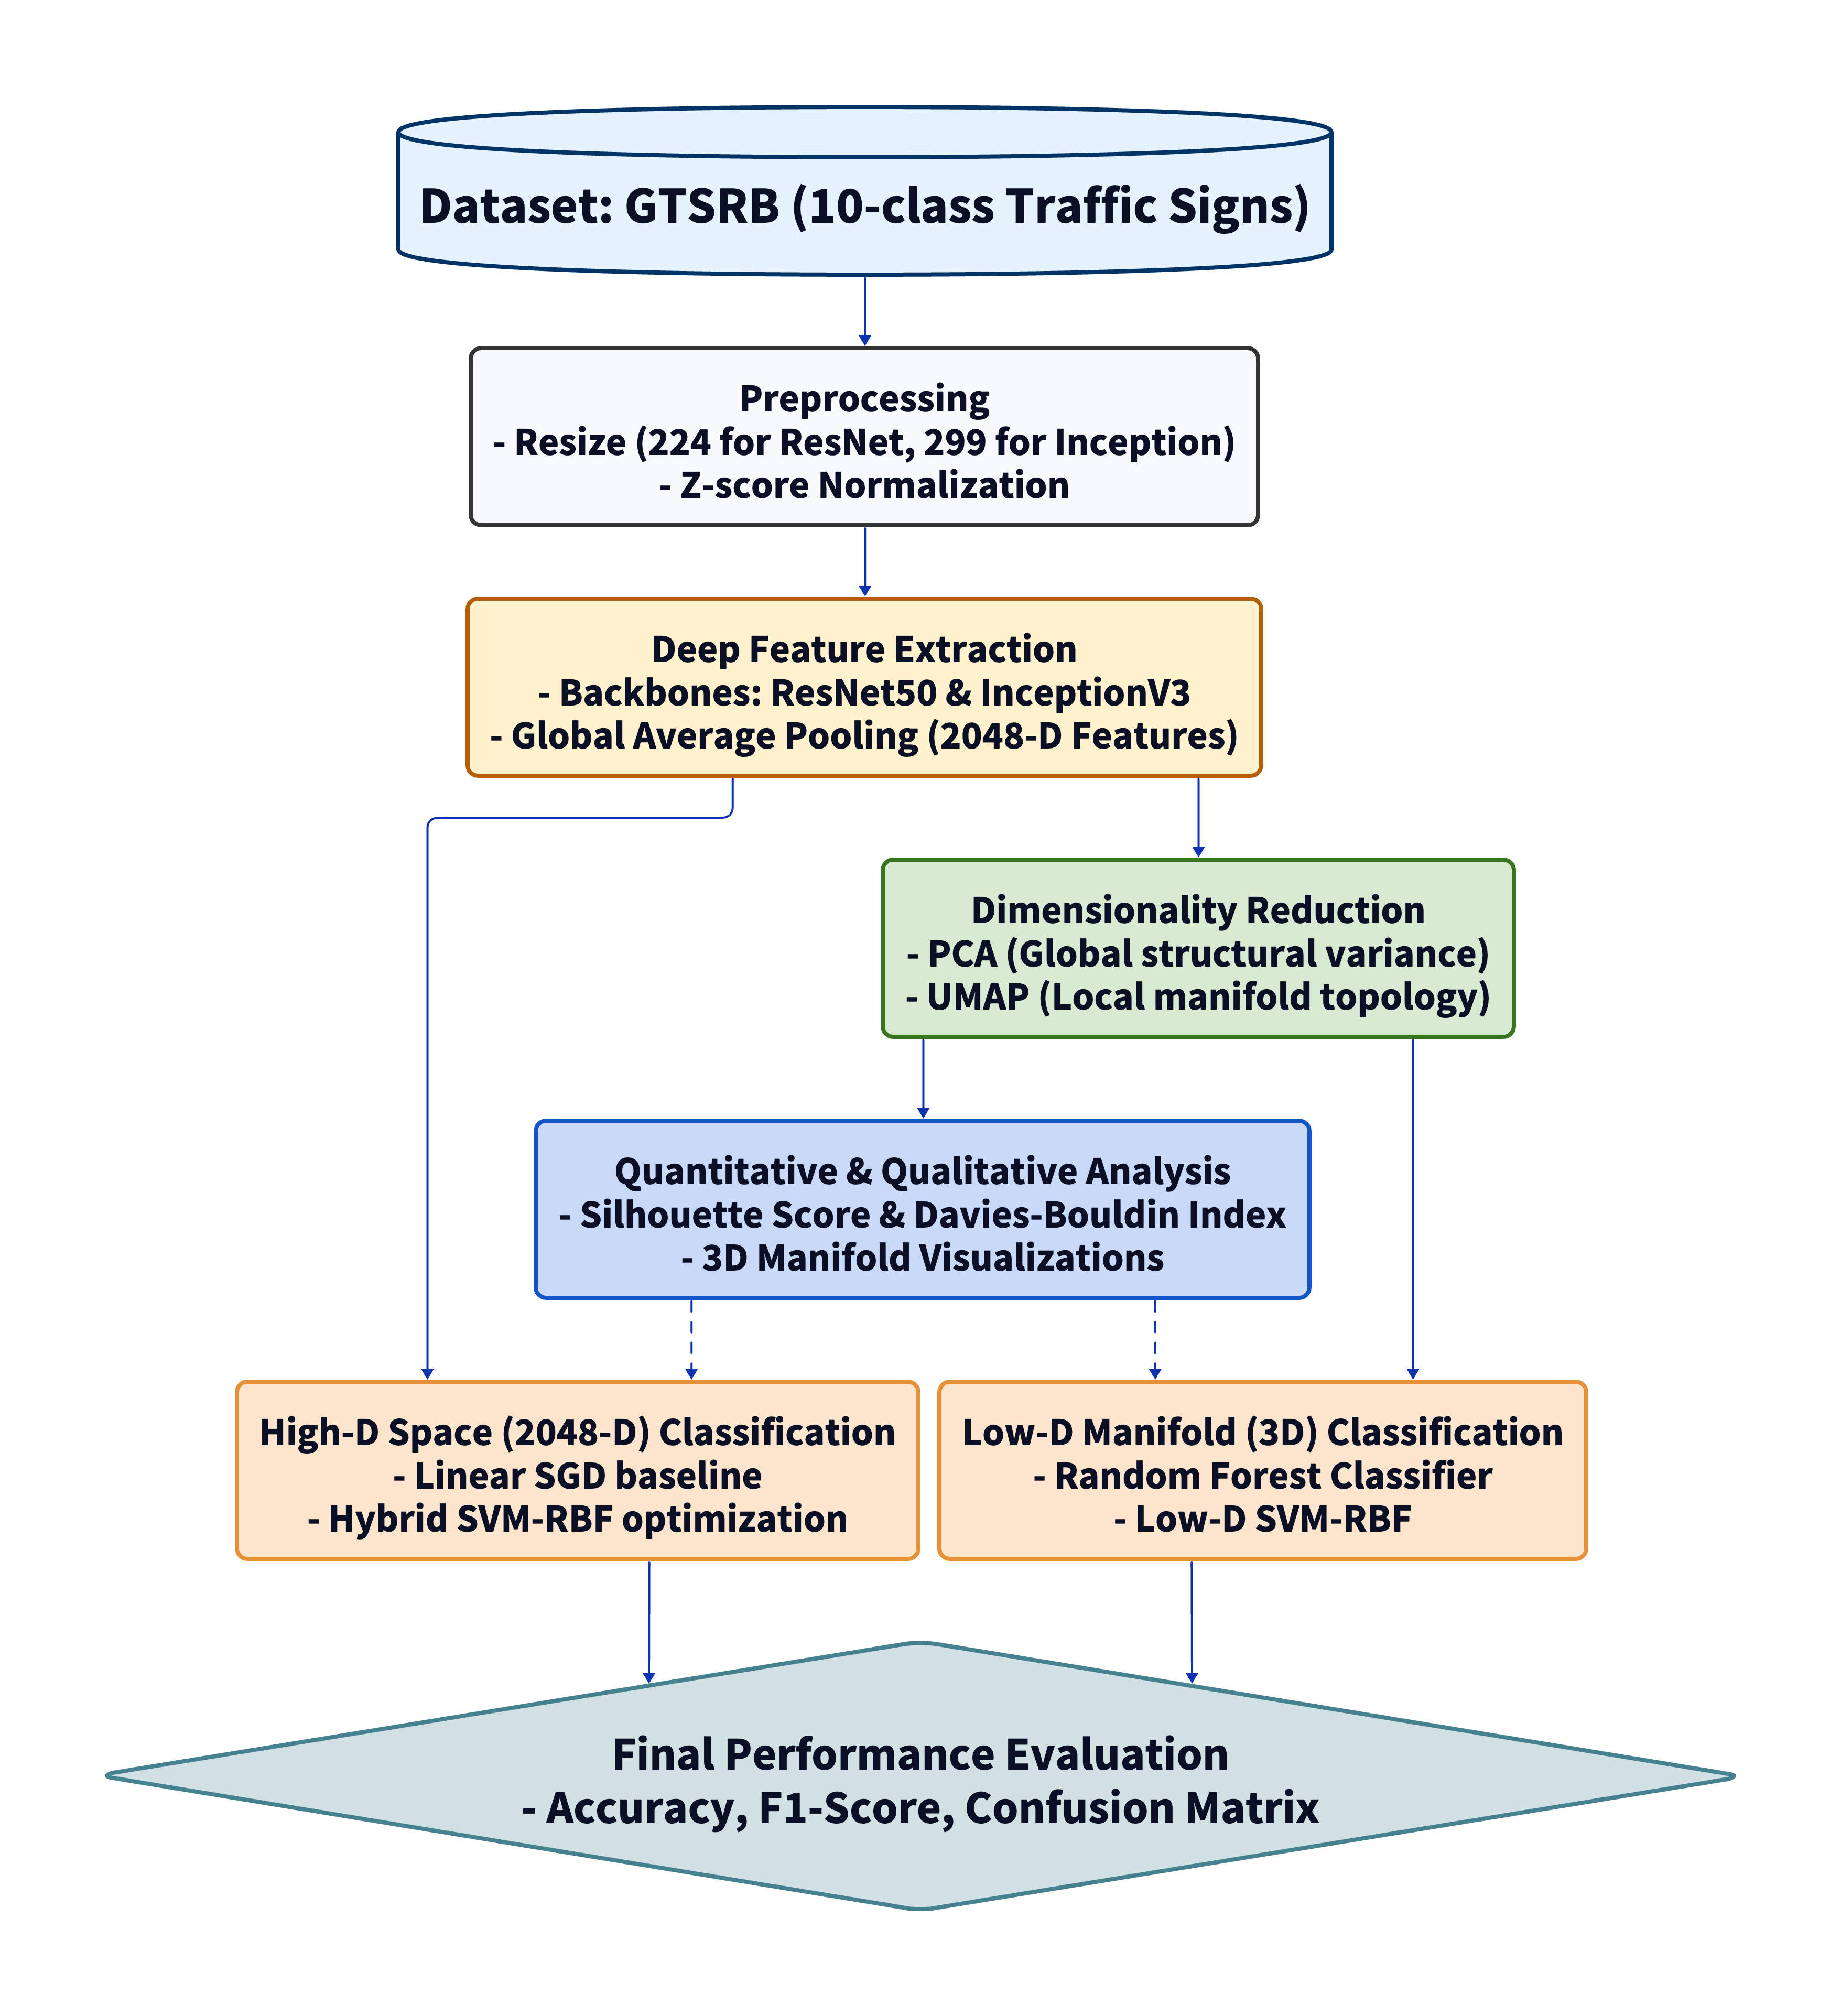
\includegraphics[width=0.85\textwidth]{../reports/figures/pipeline_flow.png}
    \caption{End-to-end system architecture and data processing pipeline.}
    \label{fig:pipeline_flow}
\end{figure}

The pipeline is organized into four primary functional blocks, each addressing a specific challenge in representation learning and machine learning optimization:
\begin{enumerate}
    \item \textbf{Data Acquisition \& Preparation:} This stage focuses on the strategic subsetting of the GTSRB dataset to address inherent class imbalances and the high variance in environmental conditions (e.g., motion blur, illumination). Preprocessing ensures that the raw visual data is normalized and resized to align with the specific inductive biases of the downstream deep extractors.
    \item \textbf{Deep Representation Learning:} We employ state-of-the-art CNN backbones not as end-to-end classifiers, but as non-linear semantic encoders. These models map the high-dimensional spatial pixel space into a compact, 2048-dimensional latent manifold, intended to capture the core discriminative features of traffic sign categories.
    \item \textbf{Geometric and Topological Analysis:} To understand the structure of the learned feature space, we employ a dual dimensionality reduction strategy. This block contrasts the global variance-maximization of linear PCA with the local neighborhood-preservation of non-linear UMAP, providing a deterministic foundation for justifying the choice of classification kernels.
    \item \textbf{Dual-Track Classification Strategy:} The final stage evaluates the robustness of the learned features through two parallel tracks. By comparing performance in the original high-dimensional space against compressed 3D manifolds, we analyze the trade-offs between information density and computational efficiency, utilizing both linear SGD-SVM baselines and optimized hybrid RBF-SVM solutions.
\end{enumerate}

\section{Dataset Selection}
The German Traffic Sign Recognition Benchmark (GTSRB) \cite{gtsrb} is a multi-category classification dataset consisting of 43 distinct traffic sign classes. For the purposes of this project, we focused on the first 10 classes to build a representative and computationally efficient classification pipeline. This subset captures a variety of shapes and colors, including speed limits, mandatory, and danger signs. 

As illustrated in Figure \ref{fig:class_dist}, the sample distribution across these 10 classes remains relatively balanced, ensuring that the model training process is not heavily biased toward any particular category.

\begin{figure}[H]
    \centering
    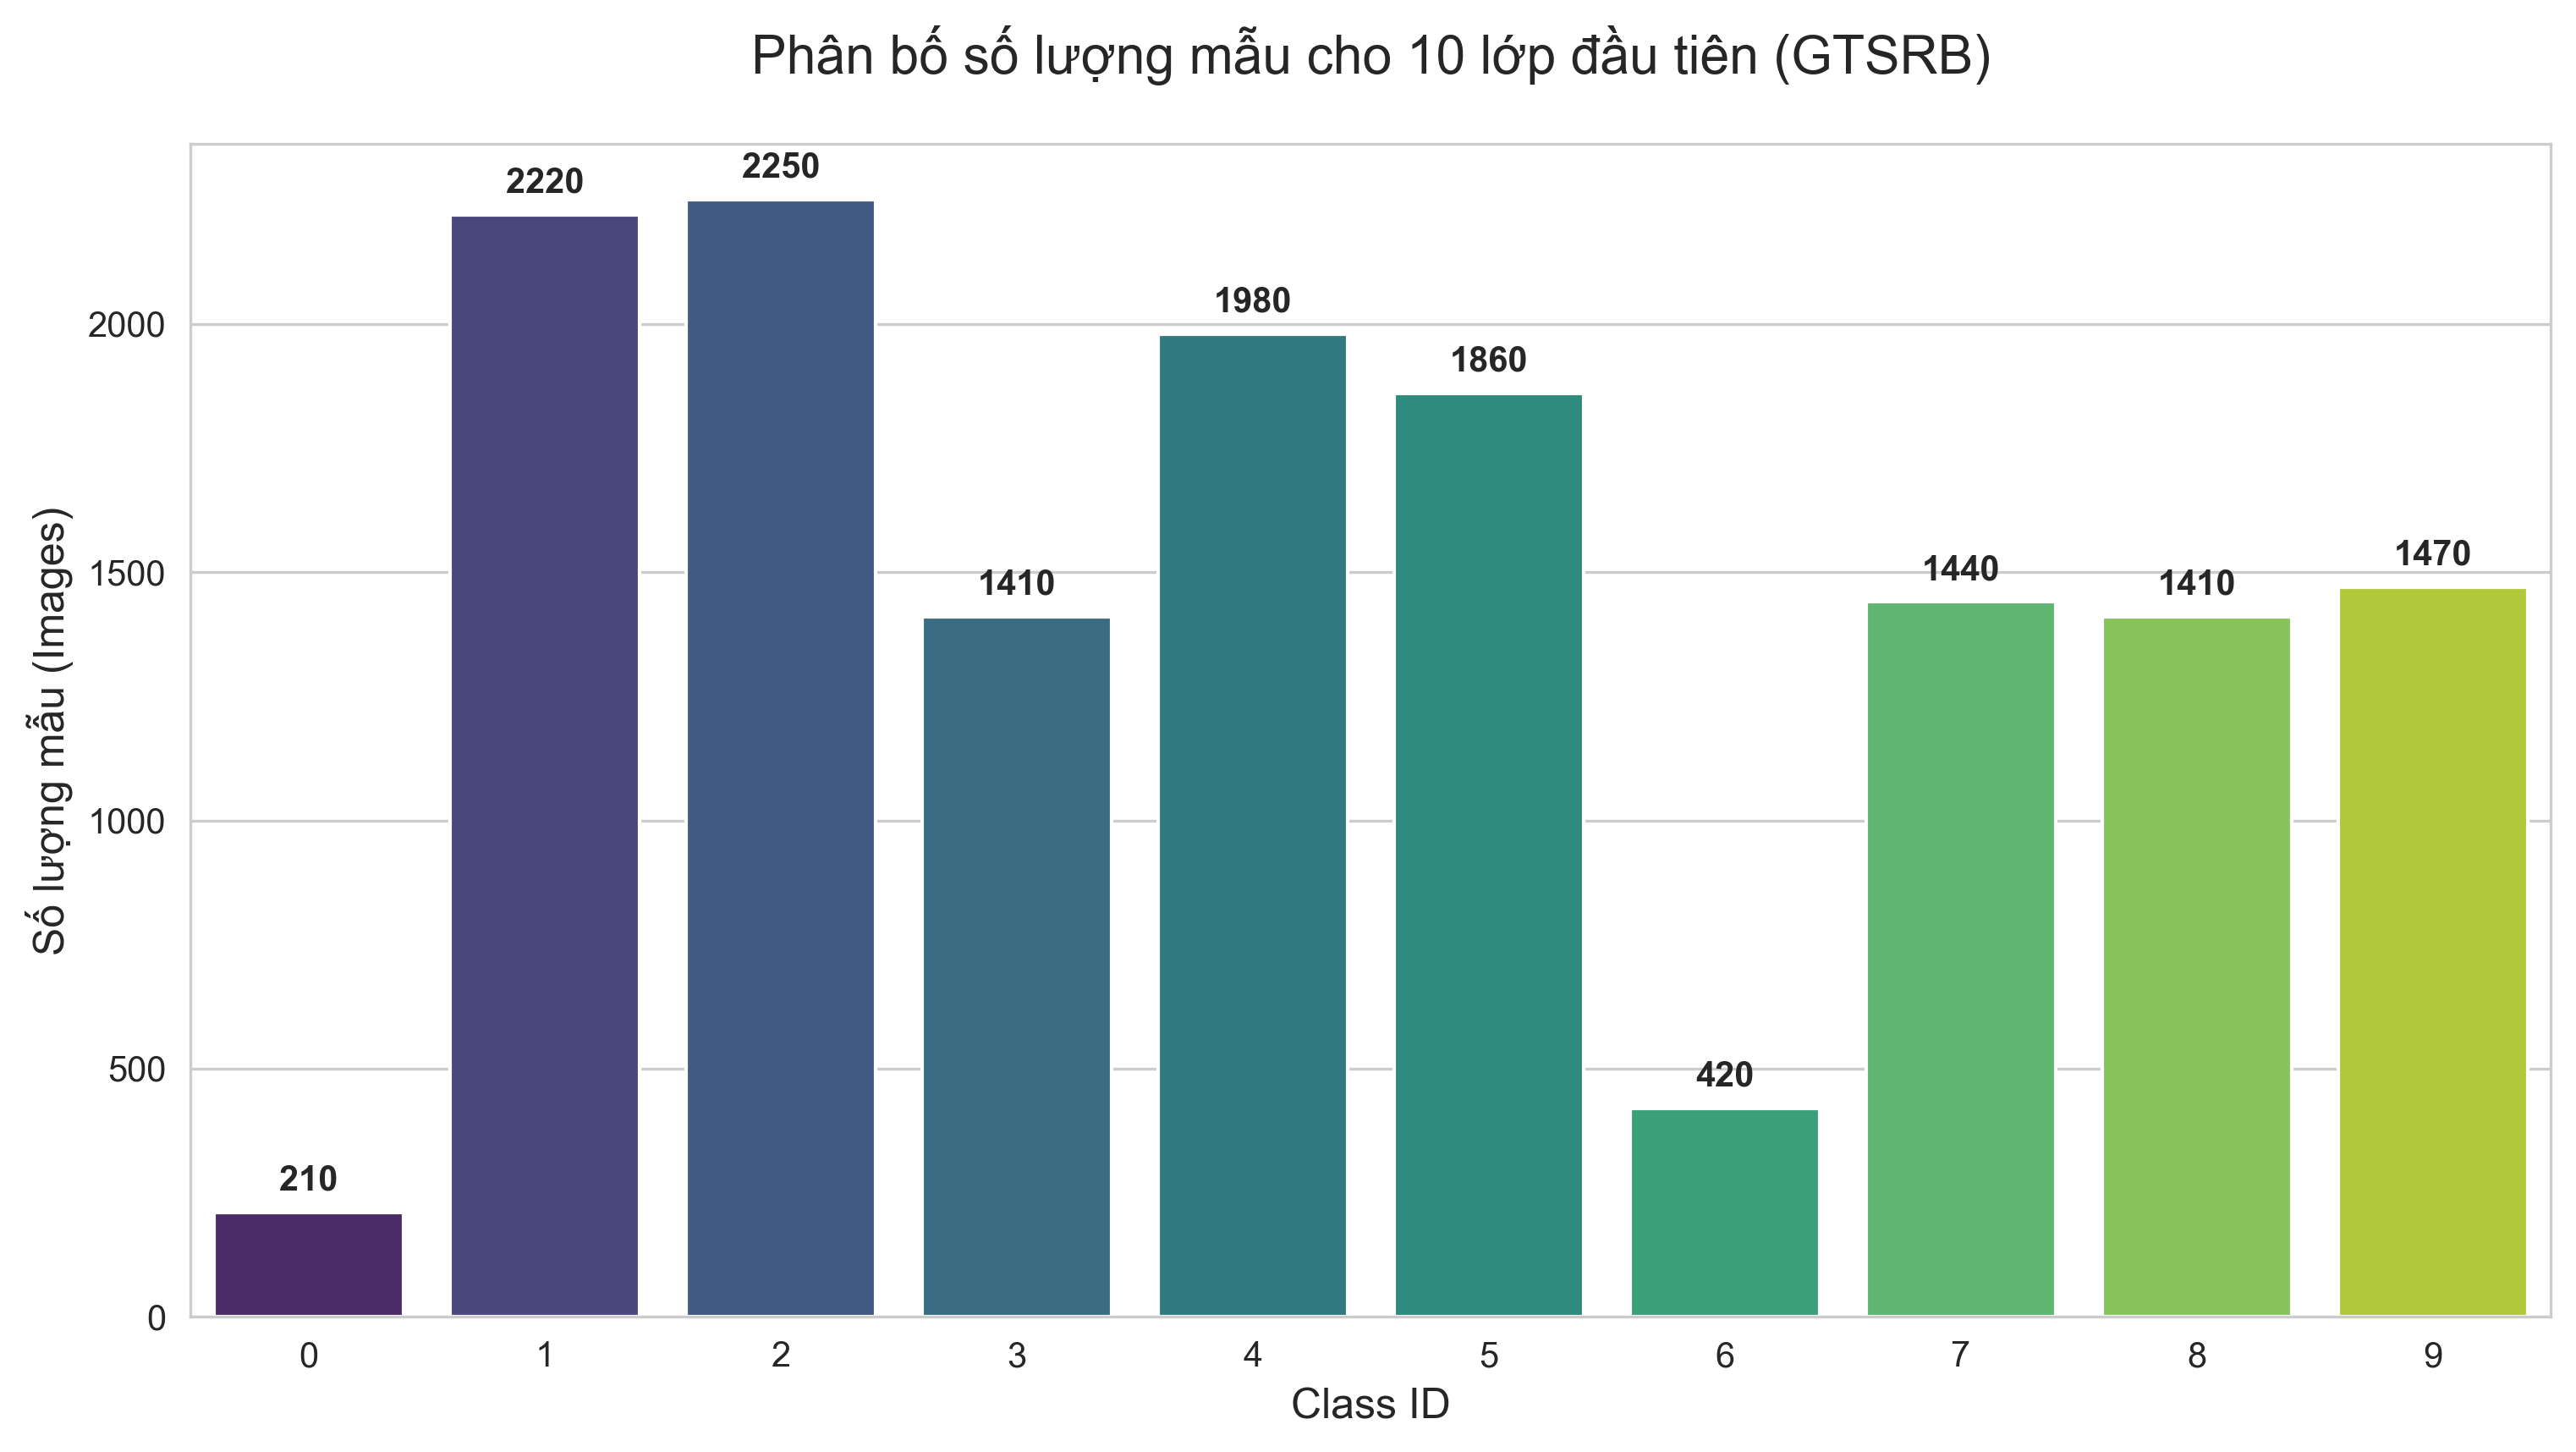
\includegraphics[width=0.8\textwidth]{../reports/figures/class_distribution_10_classes.png}
    \caption{Class distribution of the first 10 selected categories from the GTSRB dataset.}
    \label{fig:class_dist}
\end{figure}


To provide a clear understanding of the data used in this classification task, we present both the ideal class representations and the actual samples from the dataset. Figure \ref{fig:meta_ref} serves as a clean reference for each Class ID, while Figure \ref{fig:dataset_samples} displays representative real-world images from the training set. These illustrations highlight the challenges of the GTSRB dataset, including variations in lighting, motion blur, and perspective.

\begin{figure}[H]
    \centering
    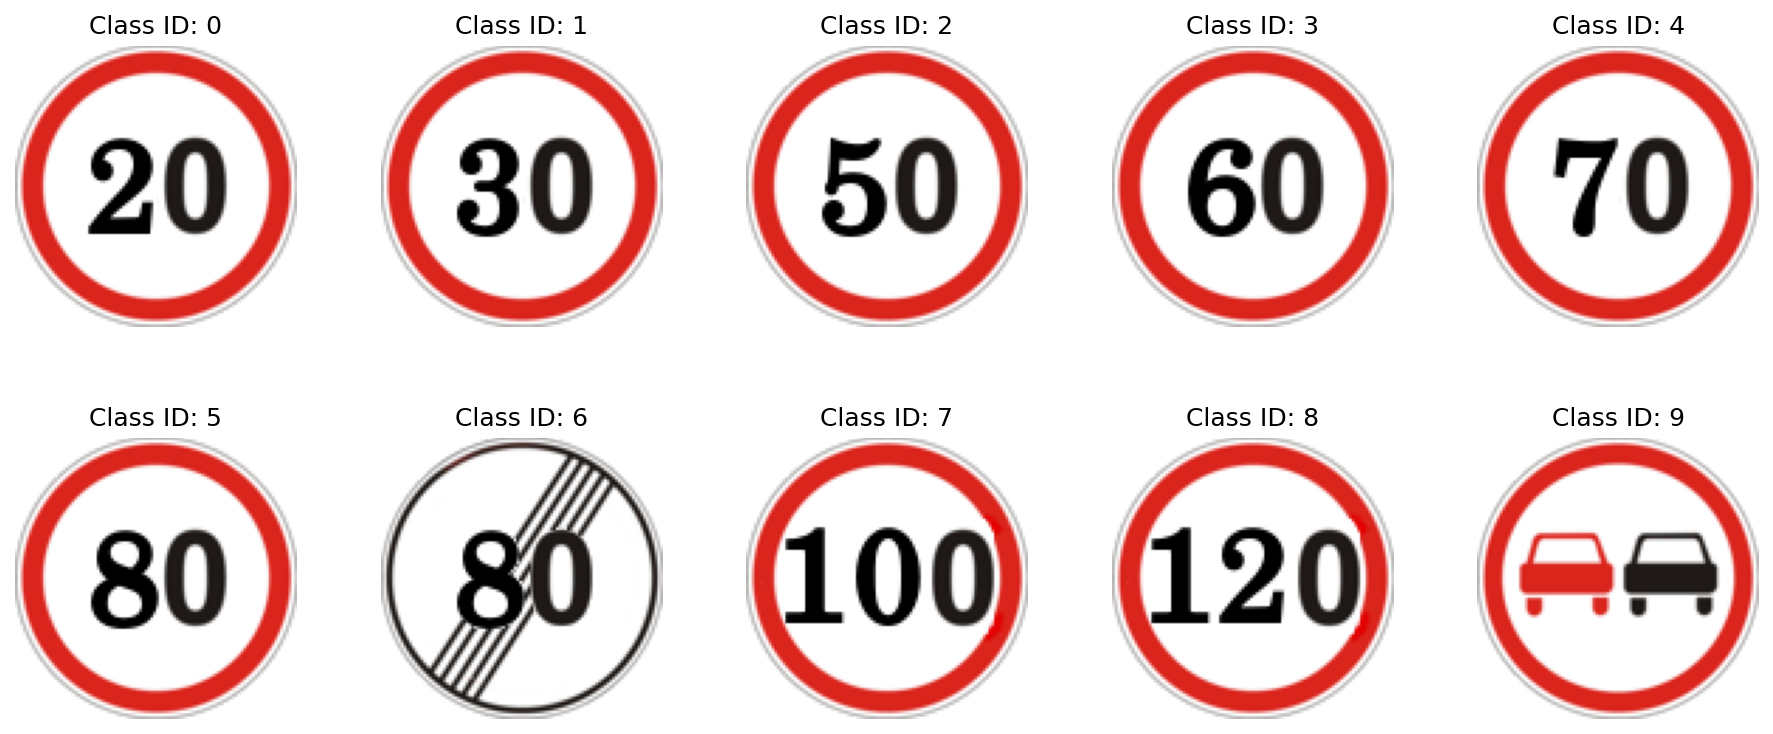
\includegraphics[width=0.85\textwidth]{../reports/figures/meta_reference.png}
    \caption{Reference icons for the 10 selected traffic sign classes (Class ID 0-9).}
    \label{fig:meta_ref}
\end{figure}

\begin{figure}[H]
    \centering
    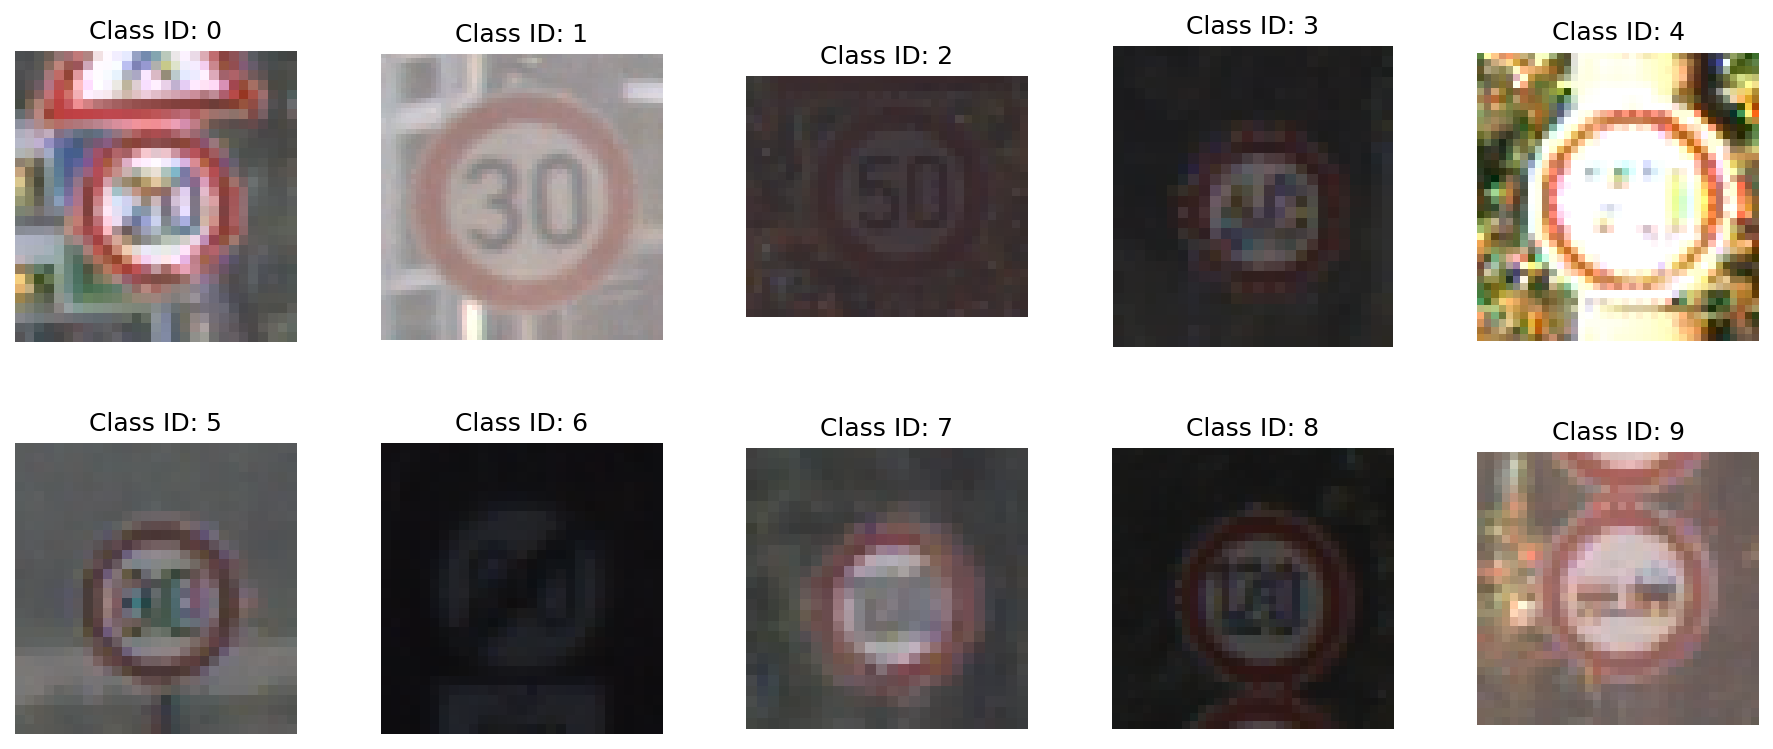
\includegraphics[width=0.85\textwidth]{../reports/figures/dataset_samples.png}
    \caption{Real-world training samples corresponding to Class IDs 0-9.}
    \label{fig:dataset_samples}
\end{figure}

\section{Feature Extraction}
This project adopts a \textbf{Transfer Learning} approach to leverage highly discriminative representations learned from the ImageNet large-scale dataset. We utilize two state-of-the-art deep convolutional neural network (CNN) architectures: ResNet50 \cite{resnet} and InceptionV3 \cite{inception}. 

\subsection{Architectural Deep-Dive}
\begin{enumerate}
    \item \textbf{ResNet50 (Residual Learning):} The core innovation of ResNet is the introduction of \textit{shortcut connections} or \textit{skip connections}. These connections allow the gradient to flow directly through the network, effectively bypassing weight layers. Mathematically, instead of learning a direct mapping $H(x)$, the network learns a residual mapping $F(x) = H(x) - x$. This architecture successfully mitigates the vanishing gradient problem, enabling the training of much deeper networks (50 layers in this case) while maintaining high representational accuracy.
    
    \item \textbf{InceptionV3 (Factorized Convolutions):} InceptionV3 focuses on computational efficiency and multi-scale feature extraction. It utilizes \textit{Inception modules} that perform convolutions with different filter sizes ($1 \times 1, 3 \times 3, 5 \times 5$) in parallel at the same level. A key technique is \textit{factorization}, such as decomposing a $7 \times 7$ convolution into two $1 \times 7$ and $7 \times 1$ filters, which reduces parameters without losing spatial information. This allows the model to capture both fine-grained and global patterns in traffic signs.
\end{enumerate}

To function as fixed feature extractors, the final fully-connected classification layers of both models are removed. We retain the convolutional base followed by a \textbf{Global Average Pooling (GAP)} layer. Unlike standard pooling, GAP computes the spatial average of each feature map across the entire $W \times H$ dimension. For both architectures, this results in a fixed-size \textbf{2048-dimensional} feature vector ($1 \times 1 \times 2048$), which serves as a compact and robust semantic summary of the input image.

The implementation is carried out using the \texttt{PyTorch} framework and the \texttt{torchvision.models} library. Raw traffic sign images are resized to $224 \times 224 \times 3$ for ResNet50 and $299 \times 299 \times 3$ for InceptionV3 to match the original training specifications.

\section{Comparative Analysis of Feature Representations}
The efficacy of the proposed classification pipeline is fundamentally contingent upon the quality of the latent representations extracted by the convolutional backbones. To rigorously evaluate the discriminative potential of these high-dimensional feature spaces prior to the final classification stage, we conduct a \textit{Quantitative Exploratory Data Analysis (EDA)} through a comparative analysis between ResNet50 and InceptionV3. This evaluation is framed as an assessment of \textbf{Representation Learning} quality, aimed at determining whether the deep extractors effectively encapsulate semantic class identities into distinct, well-separated clusters without explicit supervision during the reduction phase.

To this end, we employ a dual-framework approach to investigate the geometric and topological properties of the feature manifold:
\begin{itemize}
    \item \textbf{Linear Projection (PCA):} Assesses the global structural information and information density within the primary principal axes.
    \item \textbf{Non-linear Manifold Learning (UMAP):} Evaluates the local topological structure and the preservation of semantic class clusters in a lower-dimensional embedding.
\end{itemize}
The analysis is implemented using \texttt{Scikit-learn}, \texttt{umap-learn}, and \texttt{Matplotlib}.

\subsection{Evaluation Criteria}
In order to provide a deterministic measure of feature quality, we utilize two primary mathematical indices typically associated with unsupervised clustering. In the context of this project, these metrics serve as proxies for \textit{Class Separability}, quantifying the extent to which the deep feature manifold aligns with the ground-truth categorical labels:

\begin{enumerate}
    \item \textbf{Silhouette Score ($S$):} Measures how similar an object is to its own cluster compared to other clusters. For a data point $i$, it is defined as:
    \begin{equation}
        s(i) = \frac{b(i) - a(i)}{\max\{a(i), b(i)\}}
    \end{equation}
    where $a(i)$ is the mean intra-cluster distance and $b(i)$ is the mean nearest-cluster distance. A value closer to +1 indicates high-quality clustering, while negative values suggest points are assigned to the wrong clusters or heavy class overlap in Euclidean space. 
    
    \textit{Note:} In deep feature manifolds, negative values often reflect non-linear separability rather than poor feature quality, as Euclidean distance may fail to capture the underlying topological structure.
    
    \item \textbf{Davies-Bouldin Index ($DB$):} Evaluates the average "similarity" between clusters, focusing on the ratio of within-cluster scatter to between-cluster separation:
    \begin{equation}
        DB = \frac{1}{n} \sum_{i=1}^n \max_{j \neq i} \left( \frac{\sigma_i + \sigma_j}{d(c_i, c_j)} \right)
    \end{equation}
    where $\sigma$ represents the cluster diameter and $d(c_i, c_j)$ is the distance between cluster centroids. A lower $DB$ index signifies better class separation.

    \item \textbf{Manifold Continuity (Qualitative):} Beyond numeric scoring, we analyze the manifold structure using UMAP. A "good" representation should maintain \textit{continuity} (points of the same class stay connected) and \textit{separability} (dissimilar classes form distinct islands in the latent space).
\end{enumerate}

\subsection{Information Density Analysis (PCA-based)}
Principal Component Analysis (PCA) is employed to quantify the efficiency of featured representation. A higher concentration of variance in the initial components indicates a more discriminative and compact feature space. As shown in Table \ref{tab:pca_metrics}, ResNet50 demonstrates superior compression efficiency.

\begin{table}[H]
    \centering
    \caption{PCA Variance Distribution Comparison}
    \label{tab:pca_metrics}
    \begin{tabular}{lccc}
        \toprule
        \textbf{Metric} & \textbf{ResNet50} & \textbf{InceptionV3} & \textbf{Delta} \\
        \midrule
        PC1 (Core Variance) & \textbf{20.50\%} & 16.34\% & +4.16\% \\
        PC1-PC10 (Structural) & \textbf{51.77\%} & 47.07\% & +4.70\% \\
        Cumulative @ 200 components & \textbf{89.94\%} & 88.37\% & +1.57\% \\
        \bottomrule
    \end{tabular}
\end{table}

\begin{figure}[H]
    \centering
    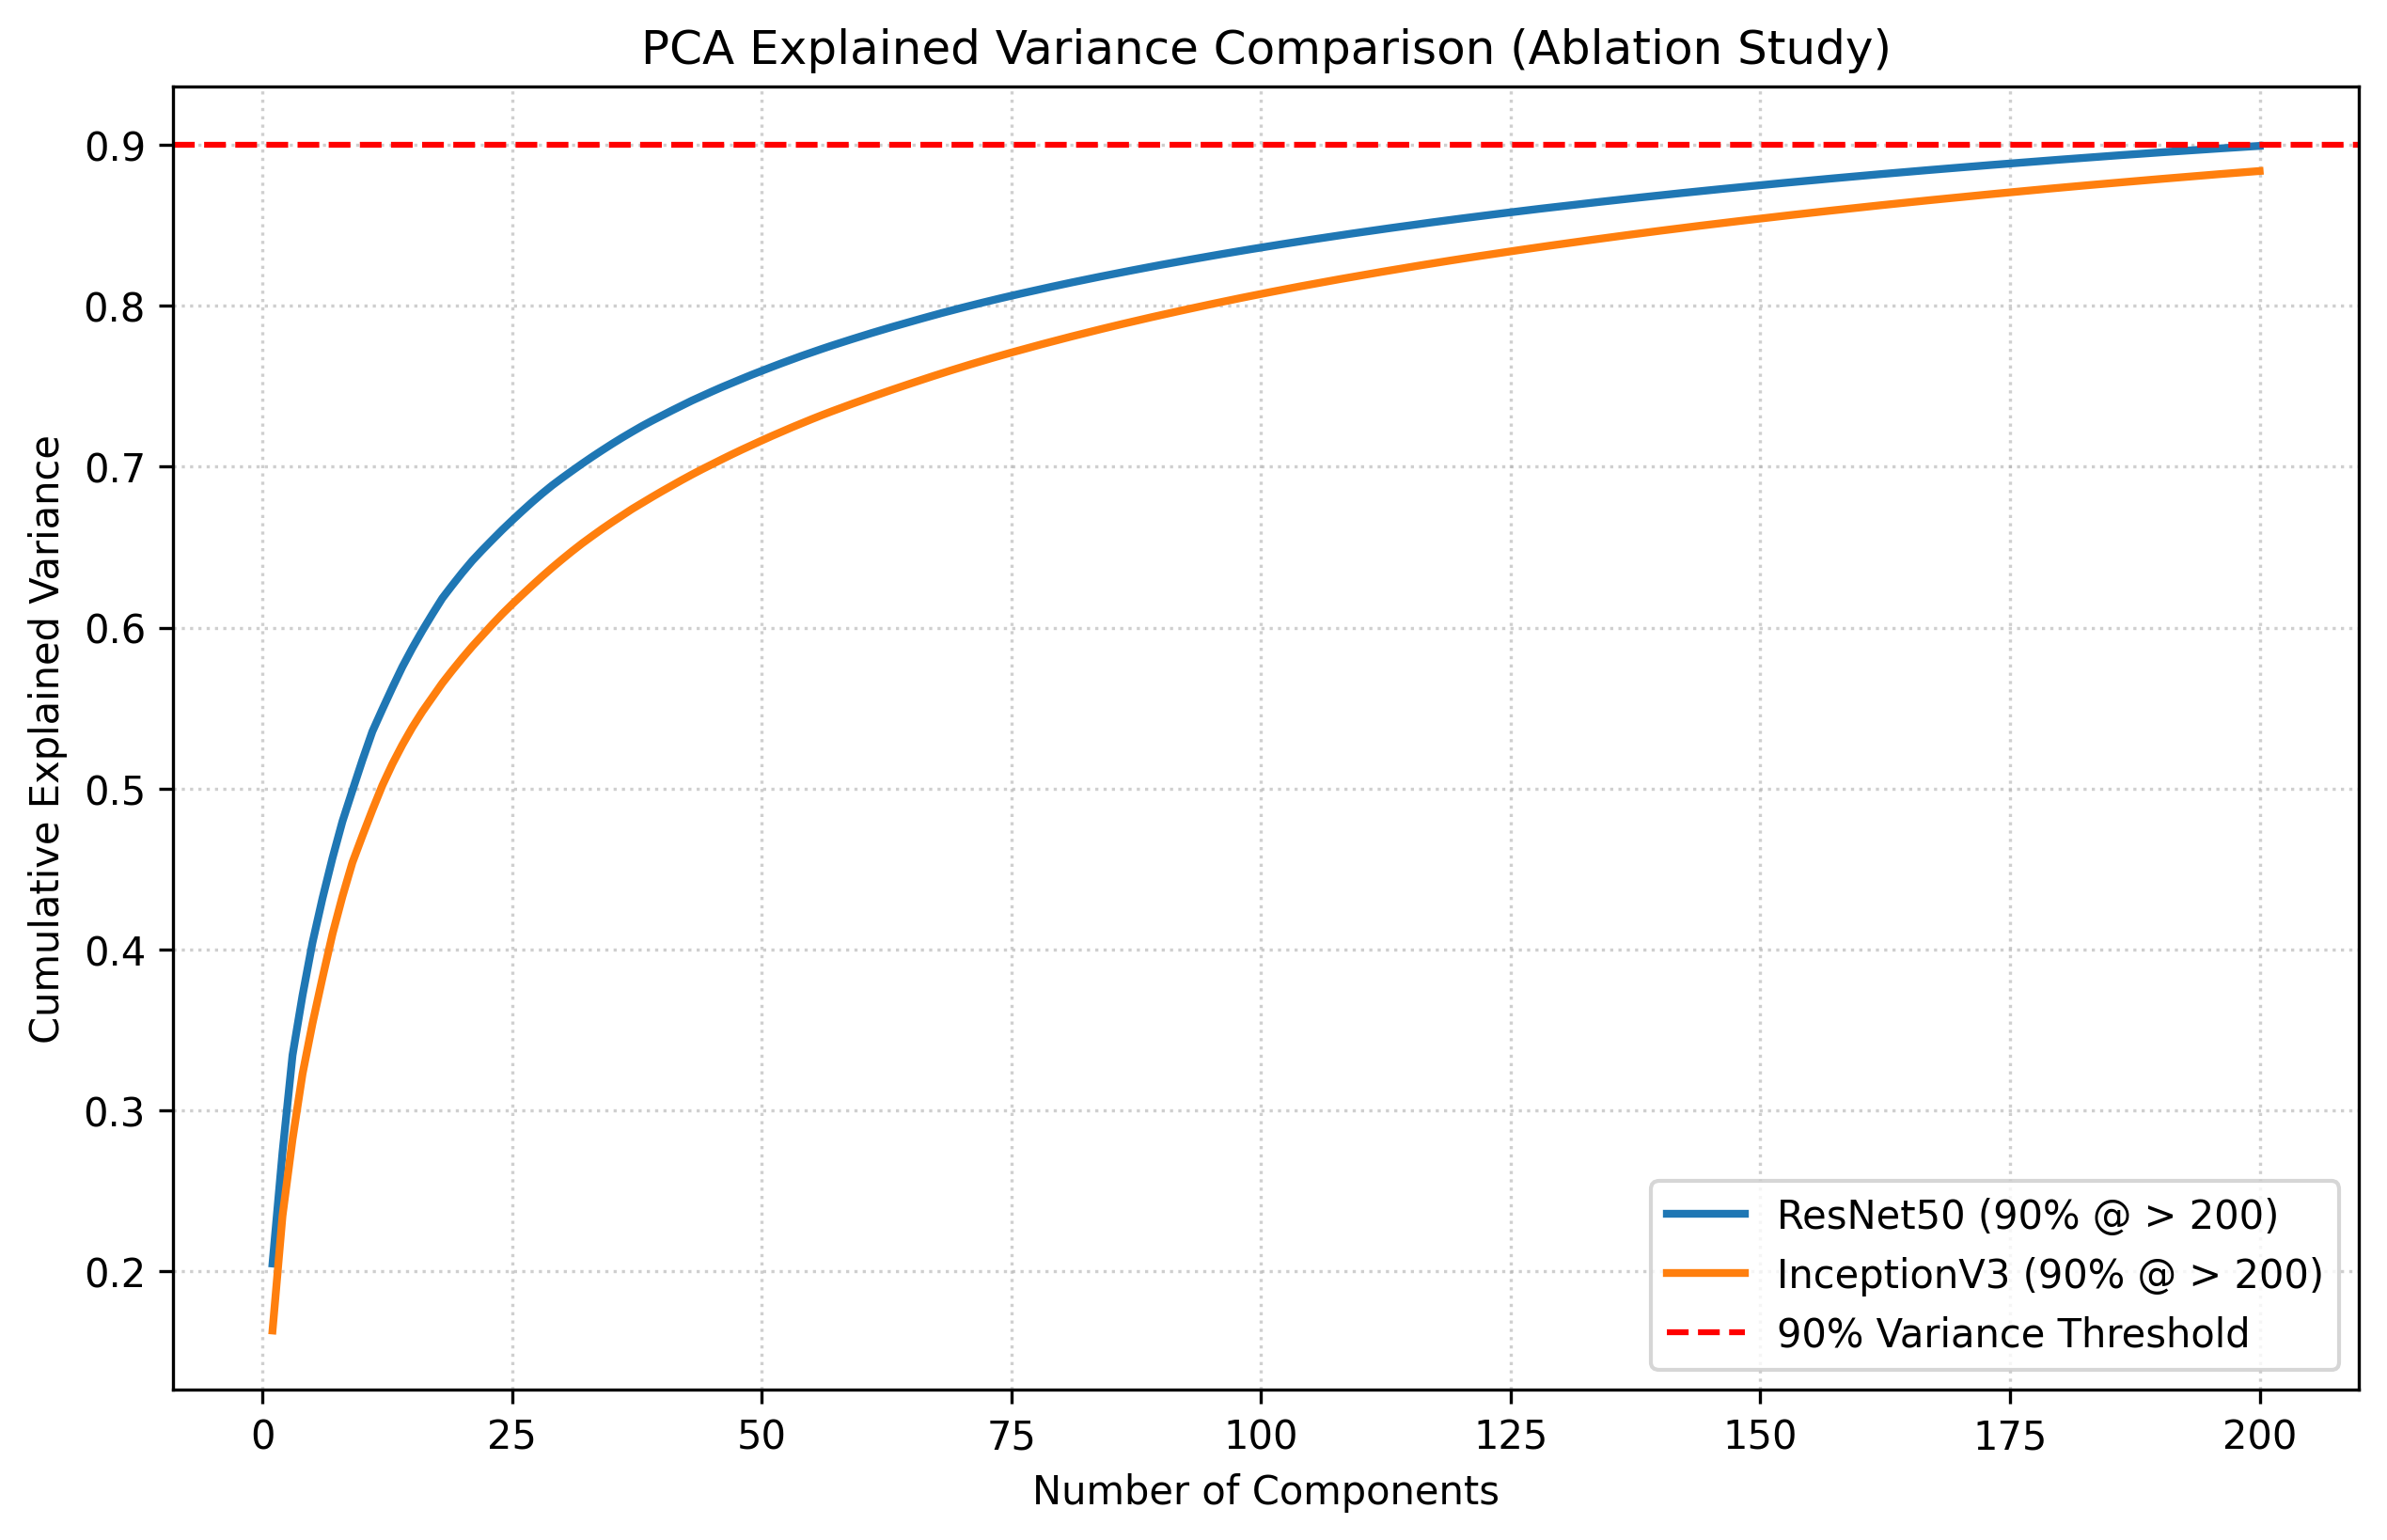
\includegraphics[width=0.8\textwidth]{../reports/figures/pca_variance_comparison.png}
    \caption{Cumulative explained variance comparison. The threshold of 200 components is selected to capture $\approx$90\% of the original information.}
    \label{fig:pca_variance_overlap}
\end{figure}

\subsection{Cluster Discriminability (UMAP-based)}
Deep features extracted from CNNs often reside on complex, non-linear manifolds in the 2048-dimensional space. While PCA identifies the axes of maximum global variance, \textbf{UMAP (Uniform Manifold Approximation and Projection)} is superior for preserving local structures and class clusters. Principal Component Analysis (PCA), a widely adopted technique for variance-maximization in high-dimensional datasets \cite{jolliffe2002}, is applied to the extracted feature vectors to reduce their dimensionality while preserving structural integrity. By constructing a fuzzy simplicial set representation of the high-dimensional data, UMAP can "unfold" the feature space into a lower dimension while maintaining class separability.

Table \ref{tab:cluster_metrics} presents the quantitative validation calculated directly on the 2048-dimensional space, confirming that ResNet50 clusters are more compact and distinct. 

\begin{table}[H]
    \centering
    \caption{Quantitative Clustering Quality Metrics (2048-D)}
    \label{tab:cluster_metrics}
    \begin{tabular}{lccc}
        \toprule
        \textbf{Metric} & \textbf{ResNet50} & \textbf{InceptionV3} & \textbf{Significance} \\
        \midrule
        Silhouette Score ($\uparrow$) & \textbf{-0.0084} & -0.0116 & Better intra-cluster density \\
        Davies-Bouldin Index ($\downarrow$) & \textbf{6.6661} & 6.8892 & Better cluster separation \\
        \bottomrule
    \end{tabular}
\end{table}

The emergence of negative Silhouette scores across both architectures requires careful technical interpretation. While traditional clustering theory suggests that negative values indicate misclassification or poorly defined clusters, we argue that in the context of deep feature manifolds, these results represent a \textit{topological discrepancy} rather than a lack of discriminative power. 

This phenomenon stems primarily from the inherent divergence between Euclidean distance metrics and non-Euclidean manifold geometry. Silhouette indices are intrinsically tied to Euclidean distances, yet high-dimensional deep features typically reside on low-dimensional manifolds characterized by high curvature. Consequently, semantic neighbors on a manifold may appear Euclidean-distant, while unrelated samples may be Euclidean-proximal due to the "curse of dimensionality," leading to localized numerical overlap in the high-dimensional space. Furthermore, the inherent similarity between certain traffic sign categories—most notably within the speed limit family (e.g., 30 km/h vs. 50 km/h)—results in boundary regions that are densely populated and heavily intertwined. 

Ultimately, these negative scores serve as a vital methodological justification. They provide empirical evidence that the feature space is not linearly separable via traditional distance-based partitioning, thereby explicitly necessitating the adoption of non-linear transformation strategies, such as \textit{Manifold Learning (UMAP)} and \textit{Radial Basis Function (RBF)} kernels, to resolve class boundaries that remain inaccessible to linear hyperplanes.

\begin{figure}[H]
    \centering
    \begin{subfigure}[b]{0.48\textwidth}
        \centering
        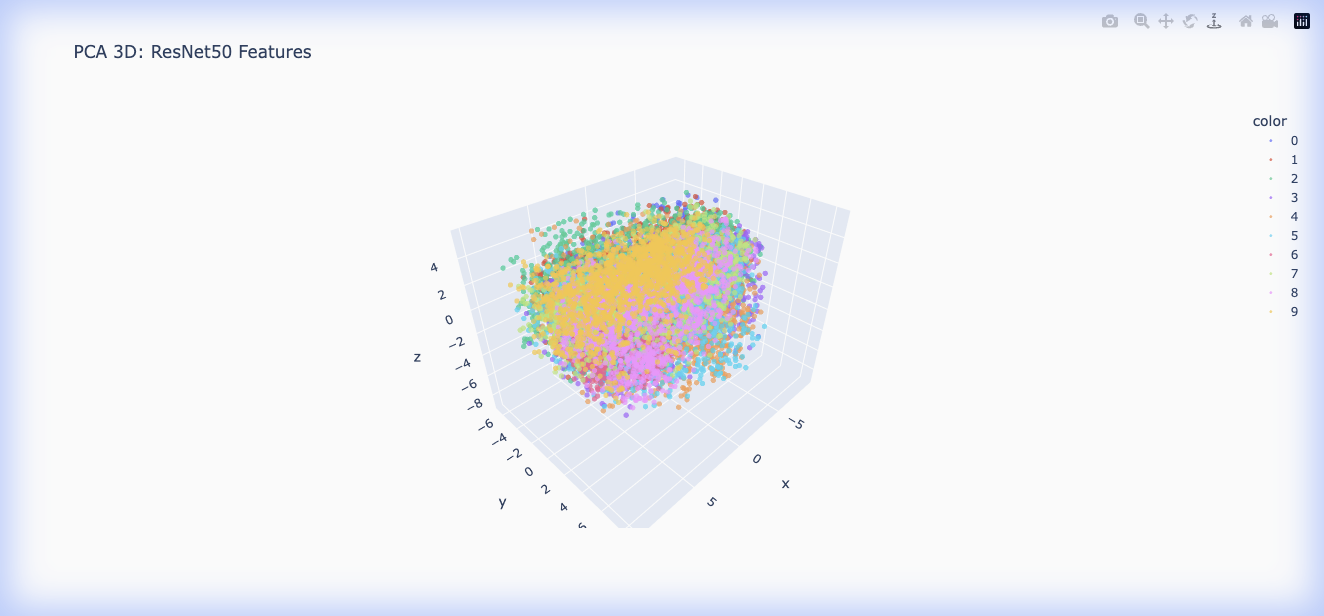
\includegraphics[width=\textwidth]{../reports/figures/pca_3d_resnet50_static.png}
        \caption{ResNet50: PCA 3D}
    \end{subfigure}
    \hfill
    \begin{subfigure}[b]{0.48\textwidth}
        \centering
        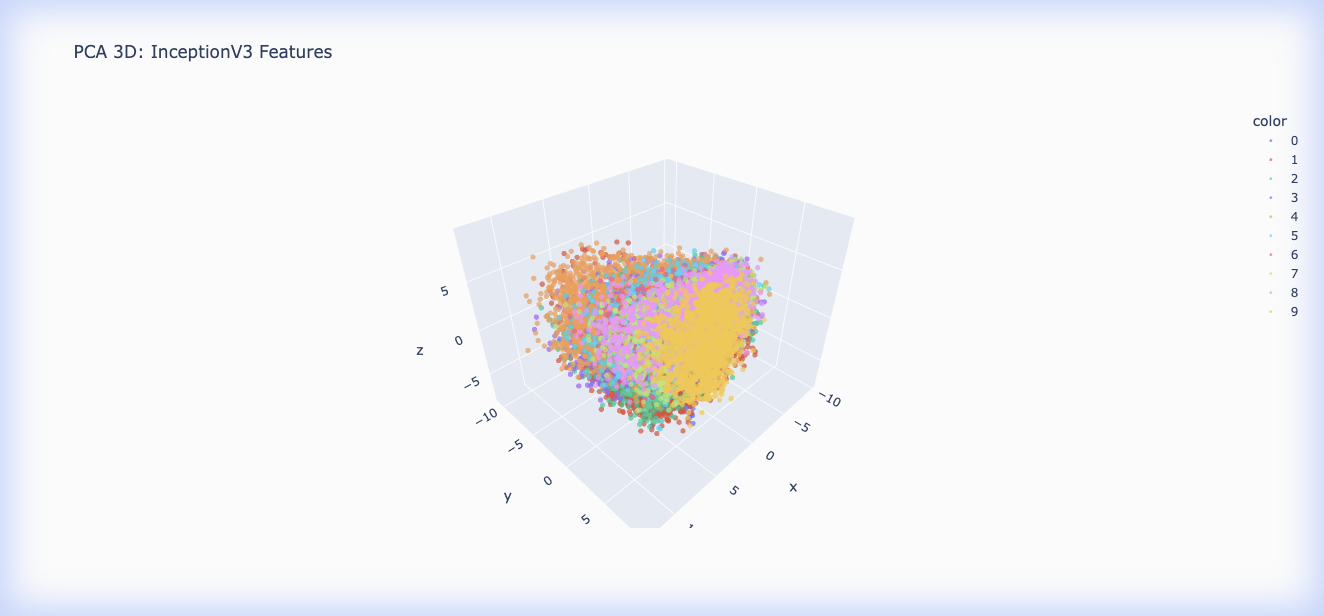
\includegraphics[width=\textwidth]{../reports/figures/pca_3d_inceptionv3_static.png}
        \caption{InceptionV3: PCA 3D}
    \end{subfigure}
    \\[20pt]
    \begin{subfigure}[b]{0.48\textwidth}
        \centering
        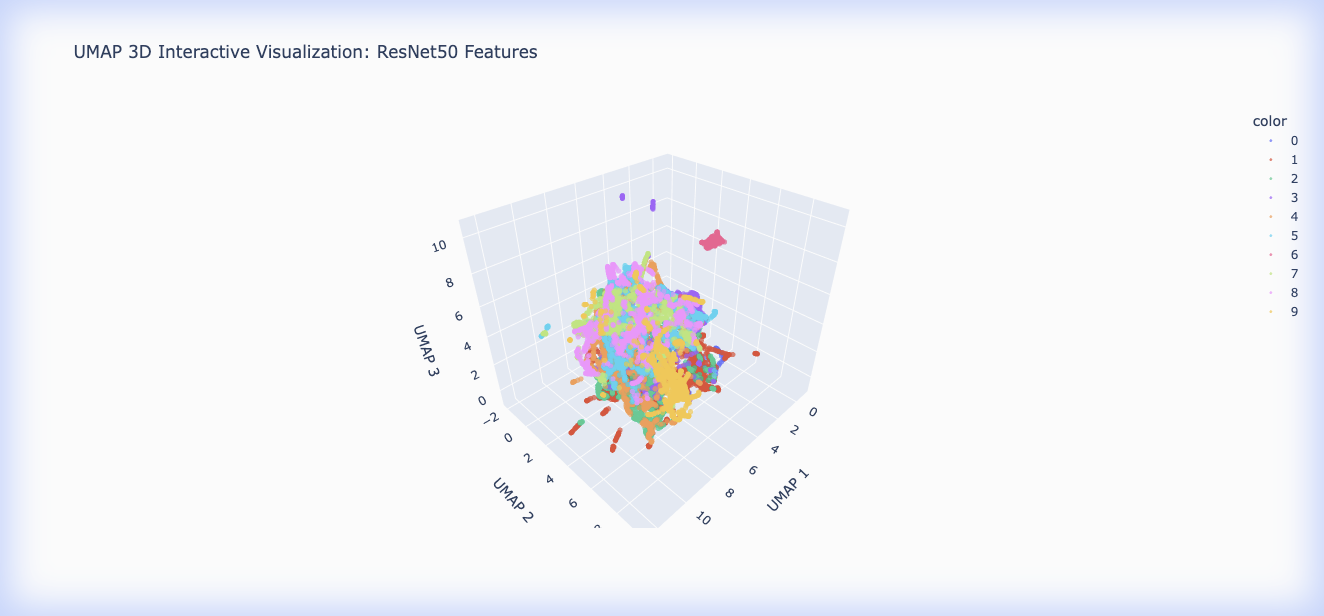
\includegraphics[width=\textwidth]{../reports/figures/umap_3d_resnet50_static.png}
        \caption{ResNet50: UMAP 3D}
    \end{subfigure}
    \hfill
    \begin{subfigure}[b]{0.48\textwidth}
        \centering
        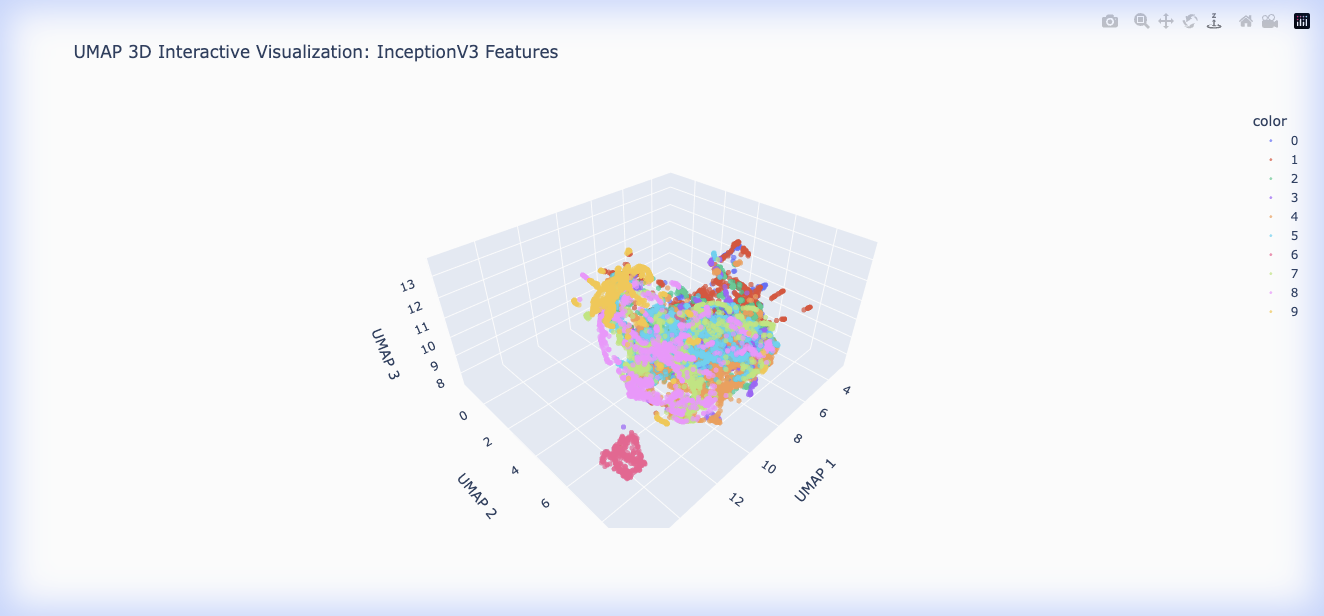
\includegraphics[width=\textwidth]{../reports/figures/umap_3d_inceptionv3_static.png}
        \caption{InceptionV3: UMAP 3D}
    \end{subfigure}
    \caption{Topological comparison of deep feature manifolds. The linear PCA projections (top) show overlapping global structures, while the non-linear UMAP manifolds (bottom) reveal well-separated, compact class clusters, justifying the use of non-linear RBF kernels.}
    \label{fig:3d_visualization}
\end{figure}

The empirical evidence from both variance analysis and clustering metrics confirms that ResNet50 provides a more structured and discriminative feature space, making it the primary candidate for achieving high accuracy in the subsequent SVM classification pipeline.

\section{Experimental Setup and Training Strategy}
The core classification task is designed to compare the robustness of linear vs. non-linear decision boundaries when applied to deep-feature spaces.

\subsection{Data Partitioning and Preprocessing}
The selected dataset of 10 traffic sign classes is partitioned into training and testing sets using the \texttt{train\_test\_split} function from the \texttt{Scikit-learn} library. We employ a stratified split ratio of \textbf{80:20} to ensure that the distribution of traffic sign categories remains consistent across both subsets. To ensure the numerical stability of the SVM optimization process, Z-score normalization is performed using the \texttt{StandardScaler} module, applied to the 2048-dimensional feature vectors:
\begin{equation}
    z = \frac{x - \mu}{\sigma}
\end{equation}
where $\mu$ and $\sigma$ are the mean and standard deviation of the training features, respectively.

\subsection{Training Strategies}
We evaluate two distinct Support Vector Machine (SVM) configurations, implemented using the \texttt{Scikit-learn} library. The data handling and matrix operations are optimized using \texttt{NumPy} and \texttt{Pandas} to ensure efficient processing of the 2048-dimensional feature sets.

\begin{enumerate}
    \item \textbf{Stochastic Gradient Descent (SGD-SVM):} To handle potential scalability requirements, we implement a linear SVM optimized via SGD with a Hinge loss function. This approach is chosen for its efficiency ($O(N)$ complexity), providing a fast yet robust baseline for linear classification task.
    \item \textbf{Radial Basis Function (RBF-SVM):} To exploit non-linear relationships, we use the RBF kernel: $K(x_i, x_j) = \exp(-\gamma ||x_i - x_j||^2)$. This configuration introduces significantly higher computational complexity ($O(N^2 \cdot D)$). Furthermore, since class probability estimation is required for downstream analysis, an \textbf{internal 5-fold cross-validation} (Platt scaling) is executed during the training phase. This hybrid approach enables the model to find more complex, non-linear decision boundaries to achieve high classification accuracy.
\end{enumerate}

\subsection{Manifold-based Classification Strategy}
Beyond the standard high-dimensional classification, we investigate the representational power of the 3D manifolds themselves. This experiment aims to determine if the local topological structures preserved by UMAP are sufficient for accurate classification. We compare three distinct algorithmic families on the 3D coordinate space:
\begin{itemize}
    \item \textbf{Random Forest Classifier (RFC):} An ensemble method that utilizes non-linear axis-aligned splits, hypothesizing that tree-based boundaries are better suited for the manifold "clusters."
    \item \textbf{Linear SGD (SGDC):} Evaluates if the 3D projection maintains linear separability.
    \item \textbf{SVM-RBF (Low-D):} Tests the efficacy of kernel-based methods in highly compressed feature spaces.
\end{itemize}
This dual-track strategy (High-D vs. Low-D) provides a comprehensive view of how information density affects model selection and decision boundary complexity.
